\chapter{Gestão de Ativos}
\label{cap-ativos}

\section{Ativos}

\textbf{Definição:} \emph{Dentro da contabilidade, ativo é um recurso econômico. Pode ser considerado qualquer coisa tangível ou intangível. Expressa bens, valores créditos, direitos e assemelhados, que podem gerar valor econômico. Formam o patrimônio de uma pessoa singular ou coletiva e são avaliados pelo seu custo.} \cite{sullivan2003}\cite{fulgencio2007} 

\textbf{Definição:} \emph{Ativo físico é algo que tem valor real ou potencial para uma organização.
Exemplos: plantas, instalações, equipamentos, estoques, ferramentas, materiais, edifícios, veículos etc.} \cite{nicolay2015}

\textbf{Definição:} \emph{Ativo é um item, coisa ou entidade que tem potencial ou valor real para uma organização.} (iso 55000)

Ativos são recursos que dão suporte as atividades realizadas por uma organização. E pelas definições acima constata-se que são intrísicos ao seu custo e também geram valor para o negócio. A troca constante desses ativos, por obsolescência, quebra ou falhas, podem gerar custos altos e despesas extras. Por isso é necessário gerí-los de forma adequada, de forma a preservá-los, a prolongar seu tempo de vida e ter uma previsão dos gastos necessários para mantê-los. 

Controlar seu ciclo de vida pode ser uma forma de prever falhas, evitá-las e assim melhorar seu desempenho e aumentar seu tempo de uso. A gestão de ativos é uma área que vem sendo valorizada exatamente porque a indústria percebeu a necessidade de diminuir os custos com reparos e substituições.

Marcio Nicolay \cite{nicolay2015} defini vida do ativo e ciclo de vida como:

\textbf{Vida do ativo:} é o período compreendido desde sua criação até o final de sua vida. Sua vida não necessariamente termina depois do descarte.

\textbf{Ciclo de vida:} são todas as etapas envolvidas na gestão de um ativo. Quantidade de etapas e duração variam de acordo com a necessidade da organização.

\subsection{Gestão de Ativos (GA)}

A norma ISO 55000 defini Gestão de Ativo como \lq\lq uma atividade coordenada de uma organização para efetuar o valor dos ativos\rq\rq, aqui a palavra \emph{atividade} pode significar a abordagem, plenejamento, planos e suas implantações. 

Gerenciamento de Ativos envolve balencear custos, oportunidades e riscos diante da perfomance desajada do ativo, para alcançar os objetivos da organização. O \cite{iam} completa dizendo que a GA habilita a aplicação de abordagens analíticas para gerenciar um ativo em diferentes estágios do seu ciclo de vida.

O Sistema de Gestão de Ativos (SGA), seria a forma de determinar políticas e objetivos e como alcançar esses objetivos. É um sistem aplicado à GA para apoiá-lo, por meio de políticas, operações, entre outros \cite{abraman}. 

Ou seja, gerir um ativo pode ser considerado a ciência de tomar decisões corretas e otimizar a entrega de valor. Um objetivo em comum é o de minimizar o custo de vida do ativo, considerando riscos na tomada de decisão.

A próxima seção irá explicar melhor a Gestão de Ativos sob a ótica da PAS 55 e da ISO 55000, as quais são normas existentes para padronizar e guiar a gestão de ativos.

\section{PAS 55 e ISO 5500x}

\begin{flushright}
	“\textit{A normalização é tecnologia consolidada, que nos
permite confiar e reproduzir infinitas vezes determinado
procedimento, seja na área industrial, seja no campo de
serviços, ou em programas de gestão, com mínimas
possibilidades de errar...
\\
...
\\
Elaborar uma norma técnica é compartilhar
conhecimento, promover a competitividade, projetar a
excelência e suas melhores consequências nos planos
econômico, social e ambiental.}”
\\
Pedro Buzatto Costa
\\
HISTÓRIA DA NORMALIZAÇÃO BRASILEIRA
\end{flushright}

A citação acima diz em poucas palavras a importância de se ter normas, padrões e especificações que possam assegurar a qualidade em diferentes áreas de conhecimento.

Na área da manutenção e gestão de ativos não é diferente. A preocupação com ativos físicos tem se tornado cada vez mais maior, pois observou-se que garantir a confiabilidade, desempenho, conservar e aumentar o tempo de vida deles pode trazer benefícios significantes, sendo um dos mais importantes, o custo, gastos que podem ser poupados.

\subsection{PAS 55}
\label{pas55}

Surgiu, em reposta a uma demanda da indútria, o documento PAS 55. Publicada em 2004 pela BSI e revisada em 2008, essa especificação é composta por 28 requisitos, considerados necessários para implantar e auditar um eficiente sistema de gestão para todo o ciclo de vida de qualquer ativo físico. A PAS 55 foi dividido em duas parte, traduzidas pela ABRAMAN como:

\begin{itemize}
	\item \textbf{Parte 1:} Especificação para a gestão otimizada de ativos físicos;
	\item \textbf{Parte 2:} Diretrizes para aplicação do PAS 55-1. 
\end{itemize} 

Sua estrutura consiste em um ciclo baseado no PDCA, como mostra a figura abaixo.

\graphicspath{{figuras/}}
\begin{figure}[h]
\centering
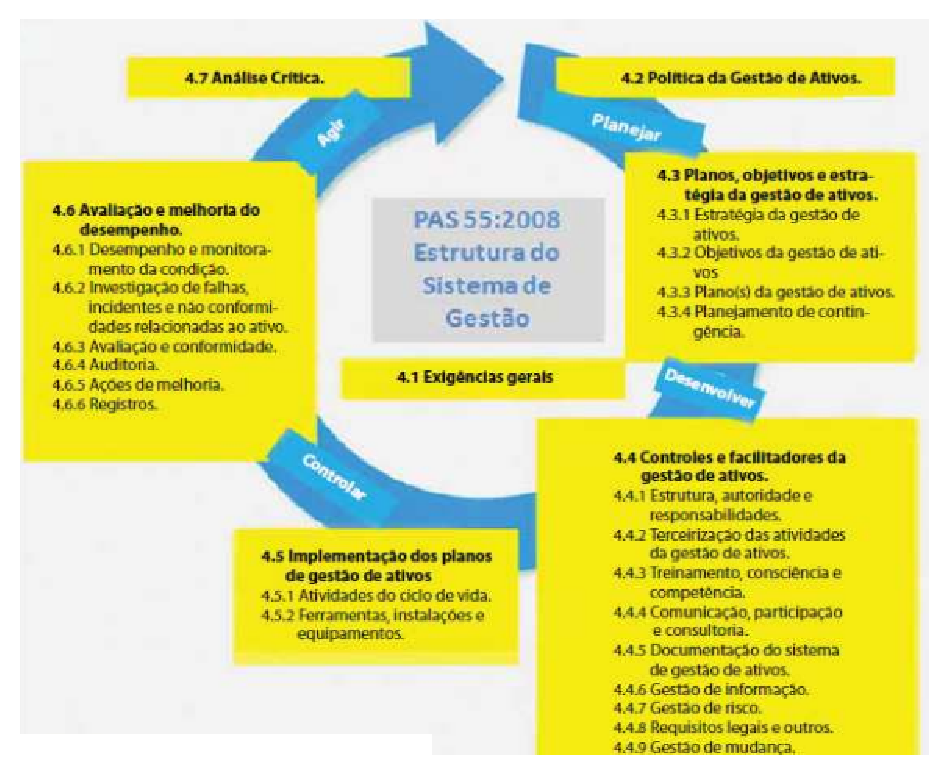
\includegraphics[width=0.8\textwidth]{figura1.eps}
\caption{Estrutura do Sistema de Gestão de Ativos PAS 55. \textbf{Fonte: BSI PAS 55-1:2008.}}
\label{estrututa_pas_55}
\end{figure}

A Figura~\ref{estrutura_pas_55} foi adaptada por \cite{valeria2013} e mostra a estrutura do Sistema de Gestão de Ativos. A PAS classifica 5 categorias de ativos:

\begin{enumerate}
	\item{Ativos Físicos}
	\item{Ativos Humanos}
	\item{Ativos de Informação}
	\item{Ativos Financeiros}
	\item{Ativos Intangíveis}
\end{enumerate}

Contudo seu escopo está focado nos \textbf{ativos físicos}. Os outros só são considerados caso estejam realacionados a eles.

Segurança, confiabilidade, disponibilidade, infraestrutura e custo são associados a atividades contidas na gestão de ativos. 

Realizar a GA é importante para, conhecer a confiabilidade e a disponibilidade dos sistemas e componentes críticos ao longo do tempo de operação, os riscos inerentes à operação e manutenção, as probabilidades de ocorrências de eventos não desejáveis que afetem a segurança das pessoas e do meio-ambiente.


\subsection{ISO-5500x}

A importânia da PAS 55 foi reconhecida quando baseada nela, em janeiro de 2014, foi aprovada a ISO-5500x, o primeiro padrão internacional para GA. 

A ISO é uma organização internacional e não gonvernamental independente, tendo adesão de 161 organismos nacionais de normalização, sendo um deles a ABNT. Seu objetivo é construir padrões internacionais relevantes para o mercado e que deêm suporte a inovação e traga soluções para desafios globais.

O conjunto de normas ISO-5500x começou a ser elaborado em 2010 sendo aprovada em 2014. Foram aprovadas então três normas \cite{abraman}:

\begin{enumerate}
	\item \textbf{ISO-55000} (Visão geral, princípios e terminologia): Nela está contida a definição de Ativos, GA e SGA, e também os termos utilizados na área. Ela descreve quatro princípios para GA, sendo eles:
		\begin{enumerate}
			\item Ativos fornecem valores para a organização e interessados.
			\item GA transforma a estratégia definida pela organização em tarefas, decisões, atividades técnicas e financeiras.
			\item Liderança e cultura do local de trabalho são determinantes da percepção de valor.
			\item GA garante que os ativos vão cumprir e desempenhar a sua função.
		\end{enumerate}
	\item \textbf{ISO-55001} (Sistemas de Gestão - Requisitos): aborda quais os requisitos necessários para um SGA ser aplicado efetivamente. Ter uma maturidade no processo de GA não faz parte do seu escopo. É estabelecido aqui que a organização inclua como o valor pode ser proporcionado pelo SGA, e não se limita ao desempenho financeiro, à gestão de risco, ao desempenho de produção e de serviços. Cabe a organização escolher os fatores relevantes, assim como a escolha dos indicadores proativos e reativos
		\begin{enumerate}
			\item Fornece princípios, requisitos e orientações para um SGA.
			\item Aborda requisitos como a implantação dos princípios de GA e a documentação de quais ativos fazem parte do SGA e são escopo do Sistema de Gestão.
			\item Integra os processos decisórios com relação aos técnicos e financeiros.
			\item Destaca a implantação de um processo decisório com foco no balanceamento entre os fatores riscos, custos e desempenho dos ativos.
		\end{enumerate}
	\item \textbf{ISO-55002} (Sistemas de Gestão - Orientações para a aplicação da ISO 55001): provê um guia para a aplicação do SGA. 
\end{enumerate}

Na Figura~\ref{termos_iso_55000} são mostrados como os principais termos encontrados na norma 55000 se relacionam.

\graphicspath{{figuras/}}
\begin{figure}[h]
\centering
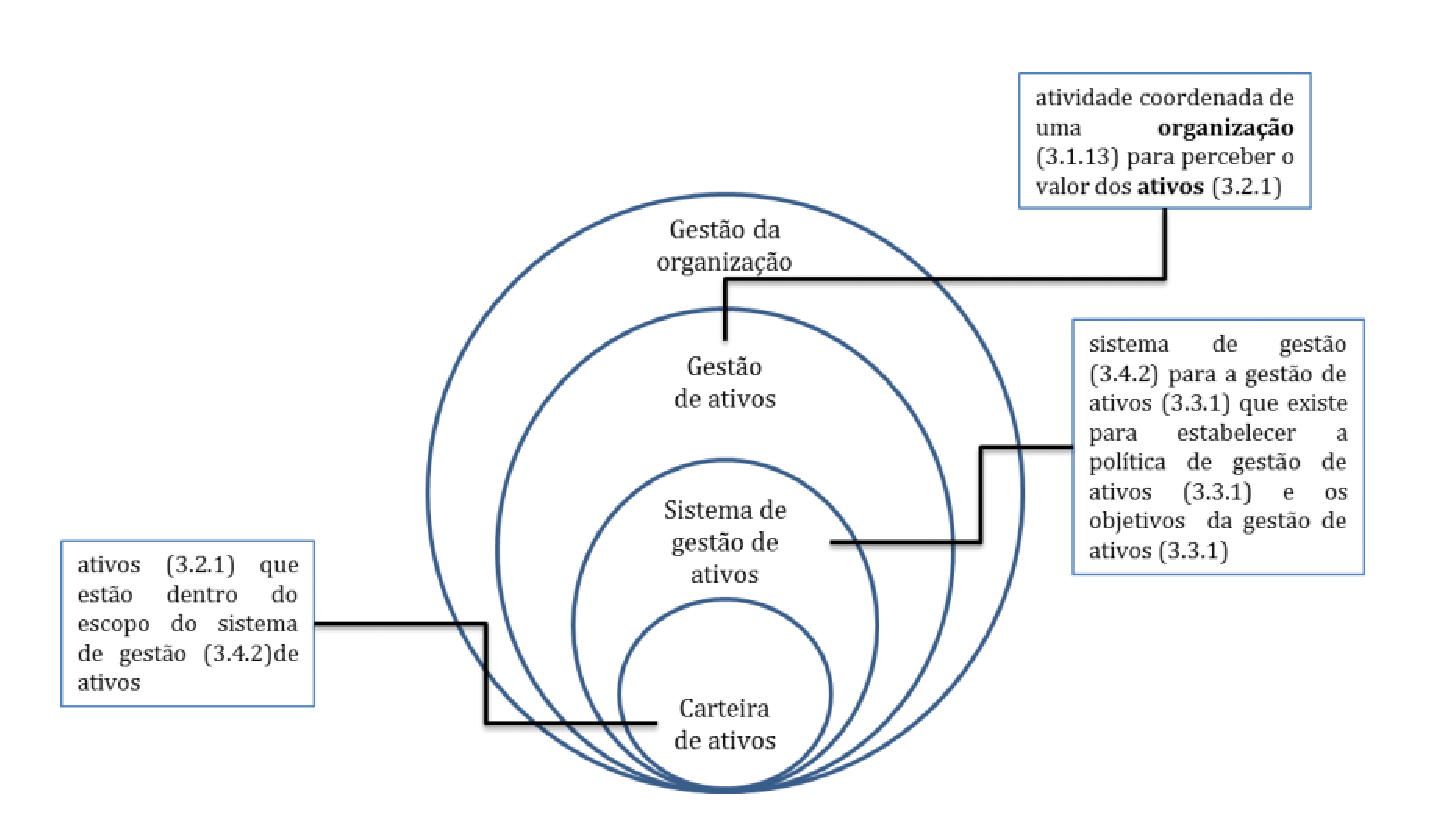
\includegraphics[width=0.8\textwidth]{termos_iso_55000.eps}
\caption{RELAÇÕES ENTRE OS PRINCIPAIS TERMOS da IS0-55000 \textbf{Fonte: Comissão de Estudo Especial de
Gestão de Ativos (ABNT/CEE-251).}}
\label{termos_iso_55000}
\end{figure}

Um dos pontos de melhoria da ISO em realação a PAS 55 Seção~\ref{pas55} é que ela fornece uma visão geral, explicando os princípios do GA, os quais podem trazer benefícios e oportunidade de alavancagem, por meio da integração com o gerenciameno de riscos e a governaça da organização. 

João Ricardo Lafraia, CMRP, Presidente da ABRAMAN diz que \lq\lq \emph{o controle eficaz e governança de ativos por organizações é essencial para realizar o valor através de gerenciamento de riscos e oportunidades, a fim de alcançar o equilíbrio desejado de custo, risco e desempenho}\rq\rq, mostrando a importância de se ter uma GA integrada com as outras partes da organização para que assim seja possível ver que uma GA efetiva e eficiente pode gerar valor de negócio na organização não só financeiro, mas também para uma melhor estruturação e realização de suas atividades.

